\chapter{Testing}
	\vspace{3mm}
	\begin{multicols}{2}
	\paragraph{}
		For our program, we felt given the size of the project, that it lent itself to smoke testing. The small nature of the project 
		(and most college projects) meant that the core functionality of the project, is largely the entire functionality.
		\newline
		\newline
		We weren’t implementing game logic, merely architectural logic which ties very neatly to smoke testing, where one does quick \& dirty 
		tests that test the major functions of a piece of software work.  Smoke testing is a methodology that "originated in the hardware 
		testing practice of turning on a new piece of hardware for the first time and considering it a success if it does not catch on fire".
		\newline
		\newline
		So after every change, we would re-compile, re-run through the project, and providing we introduced no new issues, we would move on to 
		the next feature.  As the book "Lessons Learned in Software Testing"\cite{lessons} puts it, 
		"smoke tests broadly cover product features in a limited time  ... if key features don't work or if key bugs haven't yet been fixed, your team won't waste further time installing or testing".
		\newline
		\newline
		This was assisted by the specification which required us to print out the methods and show our patterns at work. This meant that 
		we had a clear chart of the order of execution of our program and immediately highlighted any issues. The customization afforded 
		to us by Windows Presentation Foundation made such interface issues very easy to grapple with.
		\newline
		\newline
		We largely felt that black-box testing suited our needs for the project, especially if we were to go and implement more game-logic 
		at a later stage. This resulted in us making a simple set of test cases that we could quickly run through, especially in the later 
		stages of our project :

	\end{multicols}
		
		\begin{figure}[h!]
			\centering
			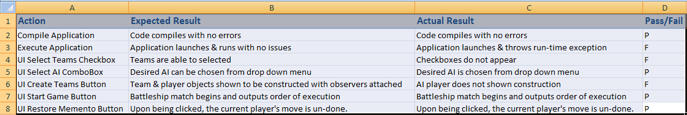
\includegraphics[width=120mm]{figures/st.png}
			  \caption{Simple test cases}
		\end{figure}


